\documentclass[a4paper]{arrowhead}

\usepackage[yyyymmdd]{datetime}
\usepackage{etoolbox}
\usepackage[utf8]{inputenc}
\usepackage{multirow}

\renewcommand{\dateseparator}{-}

\newcommand{\fparam}[1]{\textit{\textcolor{ArrowheadBlue}{#1}}}

%% Special references
\newcommand{\fref}[1]{{\textcolor{ArrowheadBlue}{\hyperref[sec:functions:#1]{#1}}}}
\newcommand{\mref}[1]{{\textcolor{ArrowheadPurple}{\hyperref[sec:model:#1]{#1}}}}
\newcommand{\pdef}[1]{{\textcolor{ArrowheadGrey}{#1 \label{sec:model:primitives:#1} \label{sec:model:primitives:#1s}}}}
\newcommand{\pref}[1]{{\textcolor{ArrowheadGrey}{\hyperref[sec:model:primitives:#1]{#1}}}}

\newrobustcmd\fsubsection[5]{
  \addtocounter{subsection}{1}
  \addcontentsline{toc}{subsection}{\protect\numberline{\thesubsection}function \textcolor{ArrowheadBlue}{#1}}
  \renewcommand*{\do}[1]{\rref{##1},\ }
  \subsection*{
    \thesubsection\quad
    #2 \textcolor{ArrowheadPurple}{#3} \\
    \small
    \hspace*{0.075\textwidth}\begin{minipage}{0.1\textwidth}
      \vspace*{1mm}
      Interface: \\
      \notblank{#4}{Input: \\}{}
      \notblank{#5}{Output: \\}{}
    \end{minipage}
    \begin{minipage}{0.825\textwidth}
      \vspace*{1mm}
      \textcolor{ArrowheadBlue}{#1} \\
      \notblank{#4}{\mref{#4} \\}{}
      \notblank{#5}{\mref{#5} \\}{}
    \end{minipage}
  }
  \label{sec:functions:#1}
}
\newrobustcmd\msubsection[2]{
  \addtocounter{subsection}{1}
  \addcontentsline{toc}{subsection}{\protect\numberline{\thesubsection}#1 \textcolor{ArrowheadPurple}{#2}}
  \subsection*{\thesubsection\quad#1 \textcolor{ArrowheadPurple}{#2}}
  \label{sec:model:#2} \label{sec:model:#2s}
}
%%

\begin{document}

%% Arrowhead Document Properties
\ArrowheadTitle{ServiceDiscovery HTTP/TLS/JSON}
\ArrowheadServiceID{register}
\ArrowheadType{Interface Design Description}
\ArrowheadTypeShort{IDD}
\ArrowheadVersion{4.3.0}
\ArrowheadDate{\today}
\ArrowheadAuthor{Szvetlin Tanyi}
\ArrowheadStatus{RELEASE}
\ArrowheadContact{szvetlin@aitia.ai}
\ArrowheadFooter{\href{www.arrowhead.eu}{www.arrowhead.eu}}
\ArrowheadSetup
%%

%% Front Page
\begin{center}
  \vspace*{1cm}
  \huge{\arrowtitle}

  \vspace*{0.2cm}
  \LARGE{\arrowtype}
  \vspace*{1cm}

%  \Large{Service ID: \textit{"\arrowid"}}
  \vspace*{\fill}

  % Front Page Image
  %\includegraphics{figures/TODO}

  \vspace*{1cm}
  \vspace*{\fill}

  % Front Page Abstract
  \begin{abstract}
    This document describes a HTTP/TLS/JSON variant of the Service Discovery service.
  \end{abstract}

  \vspace*{1cm}

  \scriptsize
  \begin{tabularx}{\textwidth}{l X}
    \raisebox{-0.5\height}{
\includegraphics[width=2cm]{figures/artemis_logo}} & {ARTEMIS Innovation Pilot Project: Arrowhead\newline
    THEME [SP1-JTI-ARTEMIS-2012-AIPP4 SP1-JTI-ARTEMIS-2012-AIPP6]\newline
    [Production and Energy System Automation Intelligent-Built environment and urban infrastructure for sustainable and friendly cities]}
  \end{tabularx}
  \vspace*{-0.2cm}
\end{center}
\newpage
%%

%% Table of Contents
\tableofcontents
\newpage
%%

\section{Overview}
\label{sec:overview}

This document describes the HTTP/TLS/JSON ServiceDiscovery service interface, which is enables autonomous service registration by systems.
Examples of this interaction is a system that has the capability to provide some kind of service. To enable other systems to use, to consume it, this service needs to be offered in the ServiceRegistry.

This document exists as a complement to the \textit{Service Discovery -- Service Description} document.
For further details about how this service is meant to be used, please consult that document.
The rest of this document describes how to realize the Service Discovery Register service using HTTP \cite{fielding2014hypertext}, TLS \cite{rescorla2018transport} and JSON \cite{bray2014json}, both in terms of its functions (Section \ref{sec:functions}) and its information model (Section \ref{sec:model}).

\newpage

\begin{figure}[ht!]
  \centering
  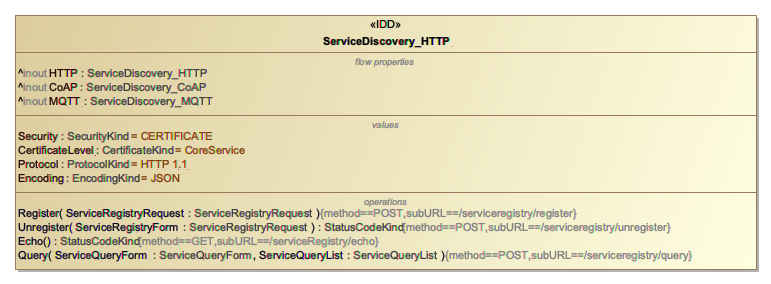
\includegraphics[width=0.8\textwidth]{figures/ServiceDiscovery-IDD}
  \caption{SysML model if the ServiceDIscovery interface, its
    operations, datamodels and implementation.}
  \label{fig:ServiceDiscovery-IDD}
\end{figure}



\section{Service Operations}
\label{sec:functions}

The interfaces of the ServiceDiscovery service, its operations, data models and implementation are provided below. An overview is found in Figure \ref{fig:ServiceDiscovery-IDD}. A SysML overview of the operation datamodels is found in Figure \ref{fig:ServiceDiscovery-datamodels}.

\begin{figure}[ht!]
  \centering
  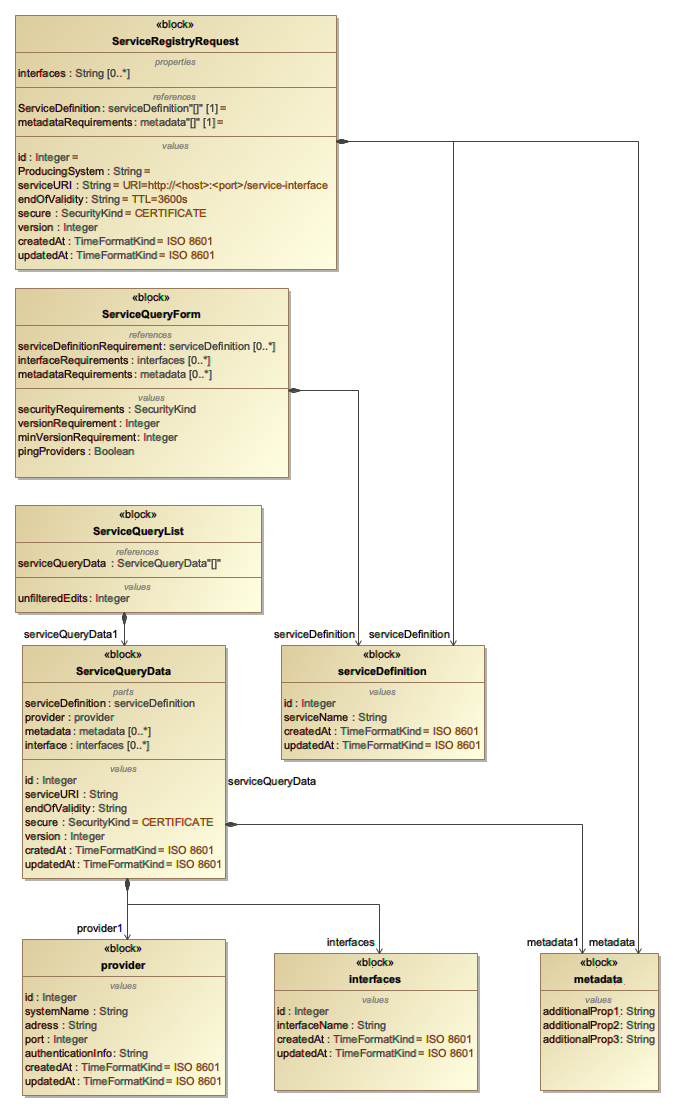
\includegraphics[width=0.8\textwidth]{figures/ServiceDiscovery-datamodels}
  \caption{A SysML models of the datamodel used by the
    ServiceDiscovery interface operations. }
  \label{fig:ServiceDiscovery-datamodels}
\end{figure}

In particular, each subsection first names the HTTP method and path used to call the function, after which it names an abstract function from the Service Discovery Register SD document, as well as input and output types.
All functions in this section respond with the HTTP status code \texttt{201 Created} if called successfully. The error codes are, \texttt{400 Bad Request} if request is malformed, \texttt{401 Unauthorized} if improper client side certificate is provided, \texttt{500 Internal Server Error} if Service Registry is unavailable.

\fsubsection{Register}{POST}{/serviceregistry/register}{ServiceRegistryRequest}{}

Called to register a service offered by the caller system, as exemplified in Listing \ref{lst:register}.

\begin{lstlisting}[language=http,label={lst:register},caption={A \fref{Register} invocation.}]
POST /serviceregistry/register HTTP/1.1

{
  "endOfValidity": "2020-12-05 12:00:00",
  "interfaces": [
    "HTTP-SECURE-JSON"
  ],
  "metadata": {
    "unit": "celsius"
  },
  "providerSystem": {
    "address": "192.168.0.101",
    "authenticationInfo": "public key of the client certificate",
    "port": 8080,
    "systemName": "exampleprovider"
  },
  "secure": "TOKEN",
  "serviceDefinition": "temperature",
  "serviceUri": "/",
  "version": 1
}
\end{lstlisting}

\begin{lstlisting}[language=http,label={lst:register_response},caption={A \fref{Register} response. Every \pref{Object} contains an id.}]
{
  "id": 14,
  "serviceDefinition": {
    "id": 13,
    "serviceDefinition": "temperature",
    "createdAt": "2020-12-01 11:59:10",
    "updatedAt": "2020-12-01 11:59:10"
  },
  "provider": {
    "id": 4,
    "systemName": "exampleprovider",
    "address": "192.168.0.101",
    "port": 8080,
    "authenticationInfo": "public key of the client certificate",
    "createdAt": "2020-12-01 11:59:10",
    "updatedAt": "2020-12-01 11:59:10"
  },
  "serviceUri": "/",
  "endOfValidity": "2020-12-05 12:00:00",
  "secure": "TOKEN",
  "metadata": {
    "unit": "celsius"
  },
  "version": 1,
  "interfaces": [
    {
      "id": 1,
      "interfaceName": "HTTP-SECURE-JSON",
      "createdAt": "2019-10-07 04:29:51",
      "updatedAt": "2019-10-07 04:29:51"
    }
  ],
  "createdAt": "2020-12-01 11:59:10",
  "updatedAt": "2020-12-01 11:59:10"
}
\end{lstlisting}

\fsubsection{Unregister}{DELETE}{/serviceregistry/unregister\\\hspace*{0.1\textwidth}?address=\iparam{\{address\}}\\\hspace*{0.1\textwidth}\&port=\iparam{\{port\}}\\\hspace*{0.1\textwidth}\&service\_definition=\iparam{\{service\_definition\}}\\\hspace*{0.1\textwidth}\&system\_name=\iparam{\{system\_name\}}}{ServiceRegistryUnregisterRequest}{}

Called to unregister a service offered by the caller system, as exemplified in Listing \ref{lst:unregister}.

\begin{lstlisting}[language=http,label={lst:unregister},caption={An \fref{Unregister} invocation.}]
DELETE /serviceregistry/unregister?address=10.0.0.0&port=8080&service_definition=temperature&system_name=mytemperaturesensor HTTP/1.1
Accept: application/json
\end{lstlisting}

\fsubsection{Query}{POST}{/serviceregistry/query}{ServiceQueryForm}{ServiceQueryList}

Called to query a service offered by a core system, as exemplified in Listing \ref{lst:query}.

\begin{lstlisting}[language=http,label={lst:query},caption={A \fref{Query} invocation.}]
POST /serviceregistry/query HTTP/1.1

{
  "interfaceRequirements": [
    "HTTP-SECURE_JSON"
  ],
  "maxVersionRequirement": 1,
  "metadataRequirements": {
    "additionalProp1": "string",
    "additionalProp2": "string",
    "additionalProp3": "string"
  },
  "minVersionRequirement": 1,
  "pingProviders": true,
  "securityRequirements": [
    "CERTIFICATE"
  ],
  "serviceDefinitionRequirement": "orchestration-service",
  "versionRequirement": 1
}

\end{lstlisting}

\begin{lstlisting}[language=http,label={lst:query_response},caption={A \fref{Query} response. Every \pref{Object} contains an id.}]
{
 "serviceQueryData": [
   {
     "id": 0,
     "serviceDefinition": {
       "id": 0,
       "serviceDefinition": "string",
       "createdAt": "string",
       "updatedAt": "string"
     },
     "provider": {
       "id": 0,
       "systemName": "string",
       "address": "string",
       "port": 0,
       "authenticationInfo": "string",
       "createdAt": "string",
       "updatedAt": "string"
     },
     "serviceUri": "string",
     "endOfValidity": "string",
     "secure": "NOT_SECURE",
     "metadata": {
       "additionalProp1": "string",
       "additionalProp2": "string",
       "additionalProp3": "string"
     },
     "version": 0,
     "interfaces": [
       {
         "id": 0,
         "interfaceName": "string",
         "createdAt": "string",
         "updatedAt": "string"
       }
     ],
     "createdAt": "string",
     "updatedAt": "string"
    }
 ],
 "unfilteredHits": 0
}
\end{lstlisting}

\fsubsection{Echo}{GET}{/serviceregistry/echo}{}{StatusCodeKind}

Called to check the core systems availability, as exemplified in Listing \ref{lst:echo}.

\begin{lstlisting}[language=http,label={lst:echo},caption={An \fref{Echo} invocation response.}]
GET /serviceregistry/echo HTTP/1.1

Got it!
\end{lstlisting}

\newpage

\section{Data Models}
\label{sec:model}

Here, all data objects that can be part of the service calls associated with this service are listed in alphabetic order.
Note that each subsection, which describes one type of object, begins with the \textit{struct} keyword, which is meant to denote a JSON \pref{Object} that must contain certain fields, or names, with values conforming to explicitly named types.
As a complement to the primary types defined in this section, there is also a list of secondary types in Section \ref{sec:model:primitives}, which are used to represent things like hashes, identifiers and texts.

\msubsection{struct}{ServiceRegistryRequest}

This structure is used to register a service offering into the Service Registry.

\begin{table}[ht!]
\begin{tabularx}{\textwidth}{| p{4.25cm} | p{3.5cm} | X |} \hline
\rowcolor{gray!33} Object Field & Value Type      & Description \\ \hline
"endofValidity"                 & \pref{DateTime} & Service is available until this UTC timestamp. \\ \hline
"interfaces"                   & \pref{Array}$<$\pref{Interface}$>$     & List of interfaces the service supports. \\ \hline
"metadata"                  & \pref{Metadata}     & Metadata \\ \hline
"providerSystem"                    & \pref{Name} & Name of the provider system. \\ \hline
"secure"                    &\pref{SecureType}  & Type of security the service uses. \\ \hline
"serviceDefinition"         &\pref{Name}        & Service Definition. \\ \hline
"serviceUri"                &\pref{URI}         & URI of the service. \\ \hline
"version"                   &\pref{Version}     & Version of the service. \\ \hline
\end{tabularx}
\end{table}

\msubsection{struct}{ServiceRegistryUnregisterRequest}

Identifies a requested Unregister call.
As the fields of this type occur only as query parameters in the \fref{Unregister} function, there is no need for it to representable as a JSON \pref{Object}.
This subsection exists only for the sake of completeness.

\msubsection{struct}{ServiceQueryForm}

This structure is used to query a service from the Service Registry.

\begin{table}[ht!]
\begin{tabularx}{\textwidth}{| p{5cm} | p{3.5cm} | X |} \hline
\rowcolor{gray!33} Object Field & Value Type      & Description \\ \hline
"interfaceRequirements"                   & \pref{Array}$<$\pref{Interface}$>$     & List of the required interfaces. \\ \hline
"maxVersionRequirement"                & \pref{Version}     & Maximum version. \\ \hline
"minVersionRequirement"                & \pref{Version}     & Minimum version. \\ \hline
"metadataRequirements"                  & \pref{Metadata}     & Metadata. \\ \hline
"pingProviders".                    & \pref{Boolean} & Checks the availability of the providers if true \\ \hline
"securityRequirements"                    &\pref{SecureType}  & Type of security. \\ \hline
"serviceDefinitionRequirement"         &\pref{Name}        & Service Definition. \\ \hline
"versionRequirement"                   &\pref{Version}     & Version of the service. \\ \hline
\end{tabularx}
\end{table}

\msubsection{struct}{Metadata}

A JSON \pref{Object} which maps \pref{String} key-value pairs.

\subsection{Primitives}
\label{sec:model:primitives}

As all messages are encoded using the JSON format \cite{bray2014json}, the following primitive constructs, part of that standard, become available.
Note that the official standard is defined in terms of parsing rules, while this list only concerns syntactic information.
Furthermore, the \pref{Object} and \pref{Array} types are given optional generic type parameters, which are used in this document to signify when pair values or elements are expected to conform to certain types. 

\begin{table}[ht!]
\begin{tabularx}{\textwidth}{| p{3cm} | X |} \hline
\rowcolor{gray!33} JSON Type & Description \\ \hline
\pdef{Value}                 & Any out of \pref{Object}, \pref{Array}, \pref{String}, \pref{Number}, \pref{Boolean} or \pref{Null}. \\ \hline
\pdef{Object}$<$A$>$         & An unordered collection of $[$\pref{String}: \pref{Value}$]$ pairs, where each \pref{Value} conforms to type A. \\ \hline
\pdef{Array}$<$A$>$          & An ordered collection of \pref{Value} elements, where each element conforms to type A. \\ \hline
\pdef{String}                & An arbitrary UTF-8 string. \\ \hline
\pdef{Number}                & Any IEEE 754 binary64 floating point number \cite{cowlishaw2019floating}, except for \textit{+Inf}, \textit{-Inf} and \textit{NaN}. \\ \hline
\pdef{Boolean}               & One out of \texttt{true} or \texttt{false}. \\ \hline
\pdef{Null}                  & Must be \texttt{null}. \\ \hline
\end{tabularx}
\end{table}

With these primitives now available, we proceed to define all the types specified in the Service Discovery Register SD document without a direct equivalent among the JSON types.
Concretely, we define the Service Discovery Register SD primitives either as \textit{aliases} or \textit{structs}.
An \textit{alias} is a renaming of an existing type, but with some further details about how it is intended to be used.
Structs are described in the beginning of the parent section.
The types are listed by name in alphabetical order.

\subsubsection{alias \pdef{DateTime} = \pref{String}}

Pinpoints a moment in time in the format of "YYYY-MM-DD HH:mm:ss", where "YYYY" denotes year (4 digits), "MM" denotes month starting from 01, "DD" denotes day starting from 01, "HH" denotes hour in the 24-hour format (00-23), "MM" denotes minute (00-59), "SS" denotes second (00-59). " " is used as separator between the date and the time.
An example of a valid date/time string is "2020-12-05 12:00:00"

\subsubsection{alias \pdef{id} = \pref{Number}}

An identifier generated for each \pref{Object} that enables to distinguish them and later to refer to a specific \pref{Object}.

\subsubsection{alias \pdef{Interface} = \pref{String}}

A \pref{String} that describes an interface in \textit{Protocol-SecurityType-MimeType} format. \textit{SecurityType} can be SECURE or INSECURE. \textit{Protocol} and \textit{MimeType} can be anything. An example of a valid interface is: "HTTPS-SECURE-JSON" or "HTTP-INSECURE-SENML".

\subsubsection{alias \pdef{Name} = \pref{String}}

A \pref{String} that is meant to be short (less than a few tens of characters) and both human and machine-readable.

\subsubsection{alias \pdef{SecureType} = \pref{String}}

A \pref{String} that describes an the security type. Possible values are \textit{NOT\_SECURE} or \textit{CERTIFICATE} or \textit{TOKEN}.

\subsubsection{alias \pdef{URI} = \pref{String}}

A \pref{String} that represents the URL subpath where the offered service is reachable, starting with a slash ("/"). An example of a valid URI is "/temperature".

\subsubsection{alias \pdef{Version} = \pref{Number}}

A \pref{Number} that represents the version of the service. And example of a valid version is: 1.

\newpage

\bibliographystyle{IEEEtran}
\bibliography{bibliography}

\newpage

\section{Revision History}
\subsection{Amendments}

\noindent\begin{tabularx}{\textwidth}{| p{1cm} | p{3cm} | p{2cm} | X | p{4cm} |} \hline
\rowcolor{gray!33} No. & Date & Version & Subject of Amendments & Author \\ \hline

1 & 2020-12-05 & 1.0.0 & & Szvetlin Tanyi \\ \hline

\end{tabularx}

\subsection{Quality Assurance}

\noindent\begin{tabularx}{\textwidth}{| p{1cm} | p{3cm} | p{2cm} | X |} \hline
\rowcolor{gray!33} No. & Date & Version & Approved by \\ \hline

1 & & & \\ \hline

\end{tabularx}

\end{document}